\graphicspath{ {../images/}}

\chapter{Preliminaries}\label{ch:preliminaries}
In this chapter, we will introduce all the necessary mathematical and quantum concepts that will be used in the rest of the thesis. It is important to understand these concepts before we move on further. We will start with the basic linear algebra concepts and then we will move on to the quantum computing concepts.
\section{Mathematics of quantum computing}
In the case of standard computers, we use boolean algebra. Quantum computing leverages the power of linear algebra. In this section, we will build upon generic linear algebra concepts and introduce some of the concepts that are specific to physics.

\subsection{Bra-ket notation}
Bra-ket notation, also known as Dirac notation plays an important role in quantum mechanics. It is a notation for vectors and matrices and is used to describe a quantum state. 

The main advantage of this notation is that enables us to easily write vector operations such as inner product, outer product, tensor product, etc.

\begin{figure}[h!]
    \begin{minipage}[b]{.5\textwidth}
    \centering
    $$\bra{\alpha} = \begin{pmatrix}
        a_1 \\
        a_2 \\
        \vdots \\
        a_n
    \end{pmatrix}$$
    \caption*{Bra}
    \end{minipage}
    \hfill
    \begin{minipage}[b]{.5\textwidth}
    \centering
    $$\ket{\beta} = \begin{pmatrix}
        b_1 & b_2 & \hdots & b_n
    \end{pmatrix}
    $$
    \caption*{Ket}
    \end{minipage}
\end{figure}

% In simple words, a bra is a column vector and a ket is a row vector. Thanks to this notation we can easily write the inner product as $\braket{\alpha}{\beta}$, the outer product as $\ket{\alpha}\bra{\beta}$ and the Kronecker product as $\ket{\alpha}\otimes\ket{\beta}$. The Kronecker product is also one of the operations that is heavily used in quantum computing. We will discuss it in more detail in the following section.
\todo{fix alignment of ket vector}
\\ \todo{consider adding a simple explanation of inner and outer product}
\\ \todo{inner product vs dot product}
\subsection{Kronecker product}
Besides the standard inner and outer product operations, the Kronecker product is another operation that is heavily used in quantum computing. It is a binary operation that combines two matrices into one larger matrix. The Kronecker product is denoted by $\otimes$ and is defined as follows:
$$A \otimes B = \begin{pmatrix}
    a_{11}B & a_{12}B & \hdots & a_{1n}B \\
    a_{21}B & a_{22}B & \hdots & a_{2n}B \\
    \vdots & \vdots & \ddots & \vdots \\
    a_{m1}B & a_{m2}B & \hdots & a_{mn}B
\end{pmatrix}$$

Essentially, we are multiplying each element of the first matrix by the second matrix. The result is a larger block matrix. Kronecker product is a specialization of the tensor product. Sometimes are these operations used interchangeably since they use the same notation $\otimes$.

\subsection{Hilbert space}
Mostly, we are used to working with finite-dimensional vector spaces. Recall that the dimension of vector space is the number of vectors required to form a basis.

In quantum computing, we work with infinite-dimensional vector spaces over $\mathbb{C}$. Virtually, Hilbert space is a standard vector space over $\mathbb{C}$, but in addition to that, it is equipped with a complete inner product.

By complete, we mean that every infinite series of vectors in Hilbert space converges to another vector in Hilbert space. $$\sum_{i=0}^{\infty}\vert a_i \vert < \infty$$
\subsection{Block sphere} 
\todo{consider covering that formula which is used to represent a qubit on a block sphere}  

\section{Introduction to quantum computing}
\textcolor{red}{TODO: consider adding motivation, maybe Moors law}

\subsection{Qubit}
Qubit is an abbreviation for quantum bit. It is a bit counterpart in quantum computing. It is a basic unit of information in quantum computers. Unlike classical bits that can hold only two values (0 or 1), qubits are more complicated. 

A qubit can be represented by the Block sphere. The Block sphere is a unit sphere. 

\begin{figure}[hbt!]
    \begin{center}
       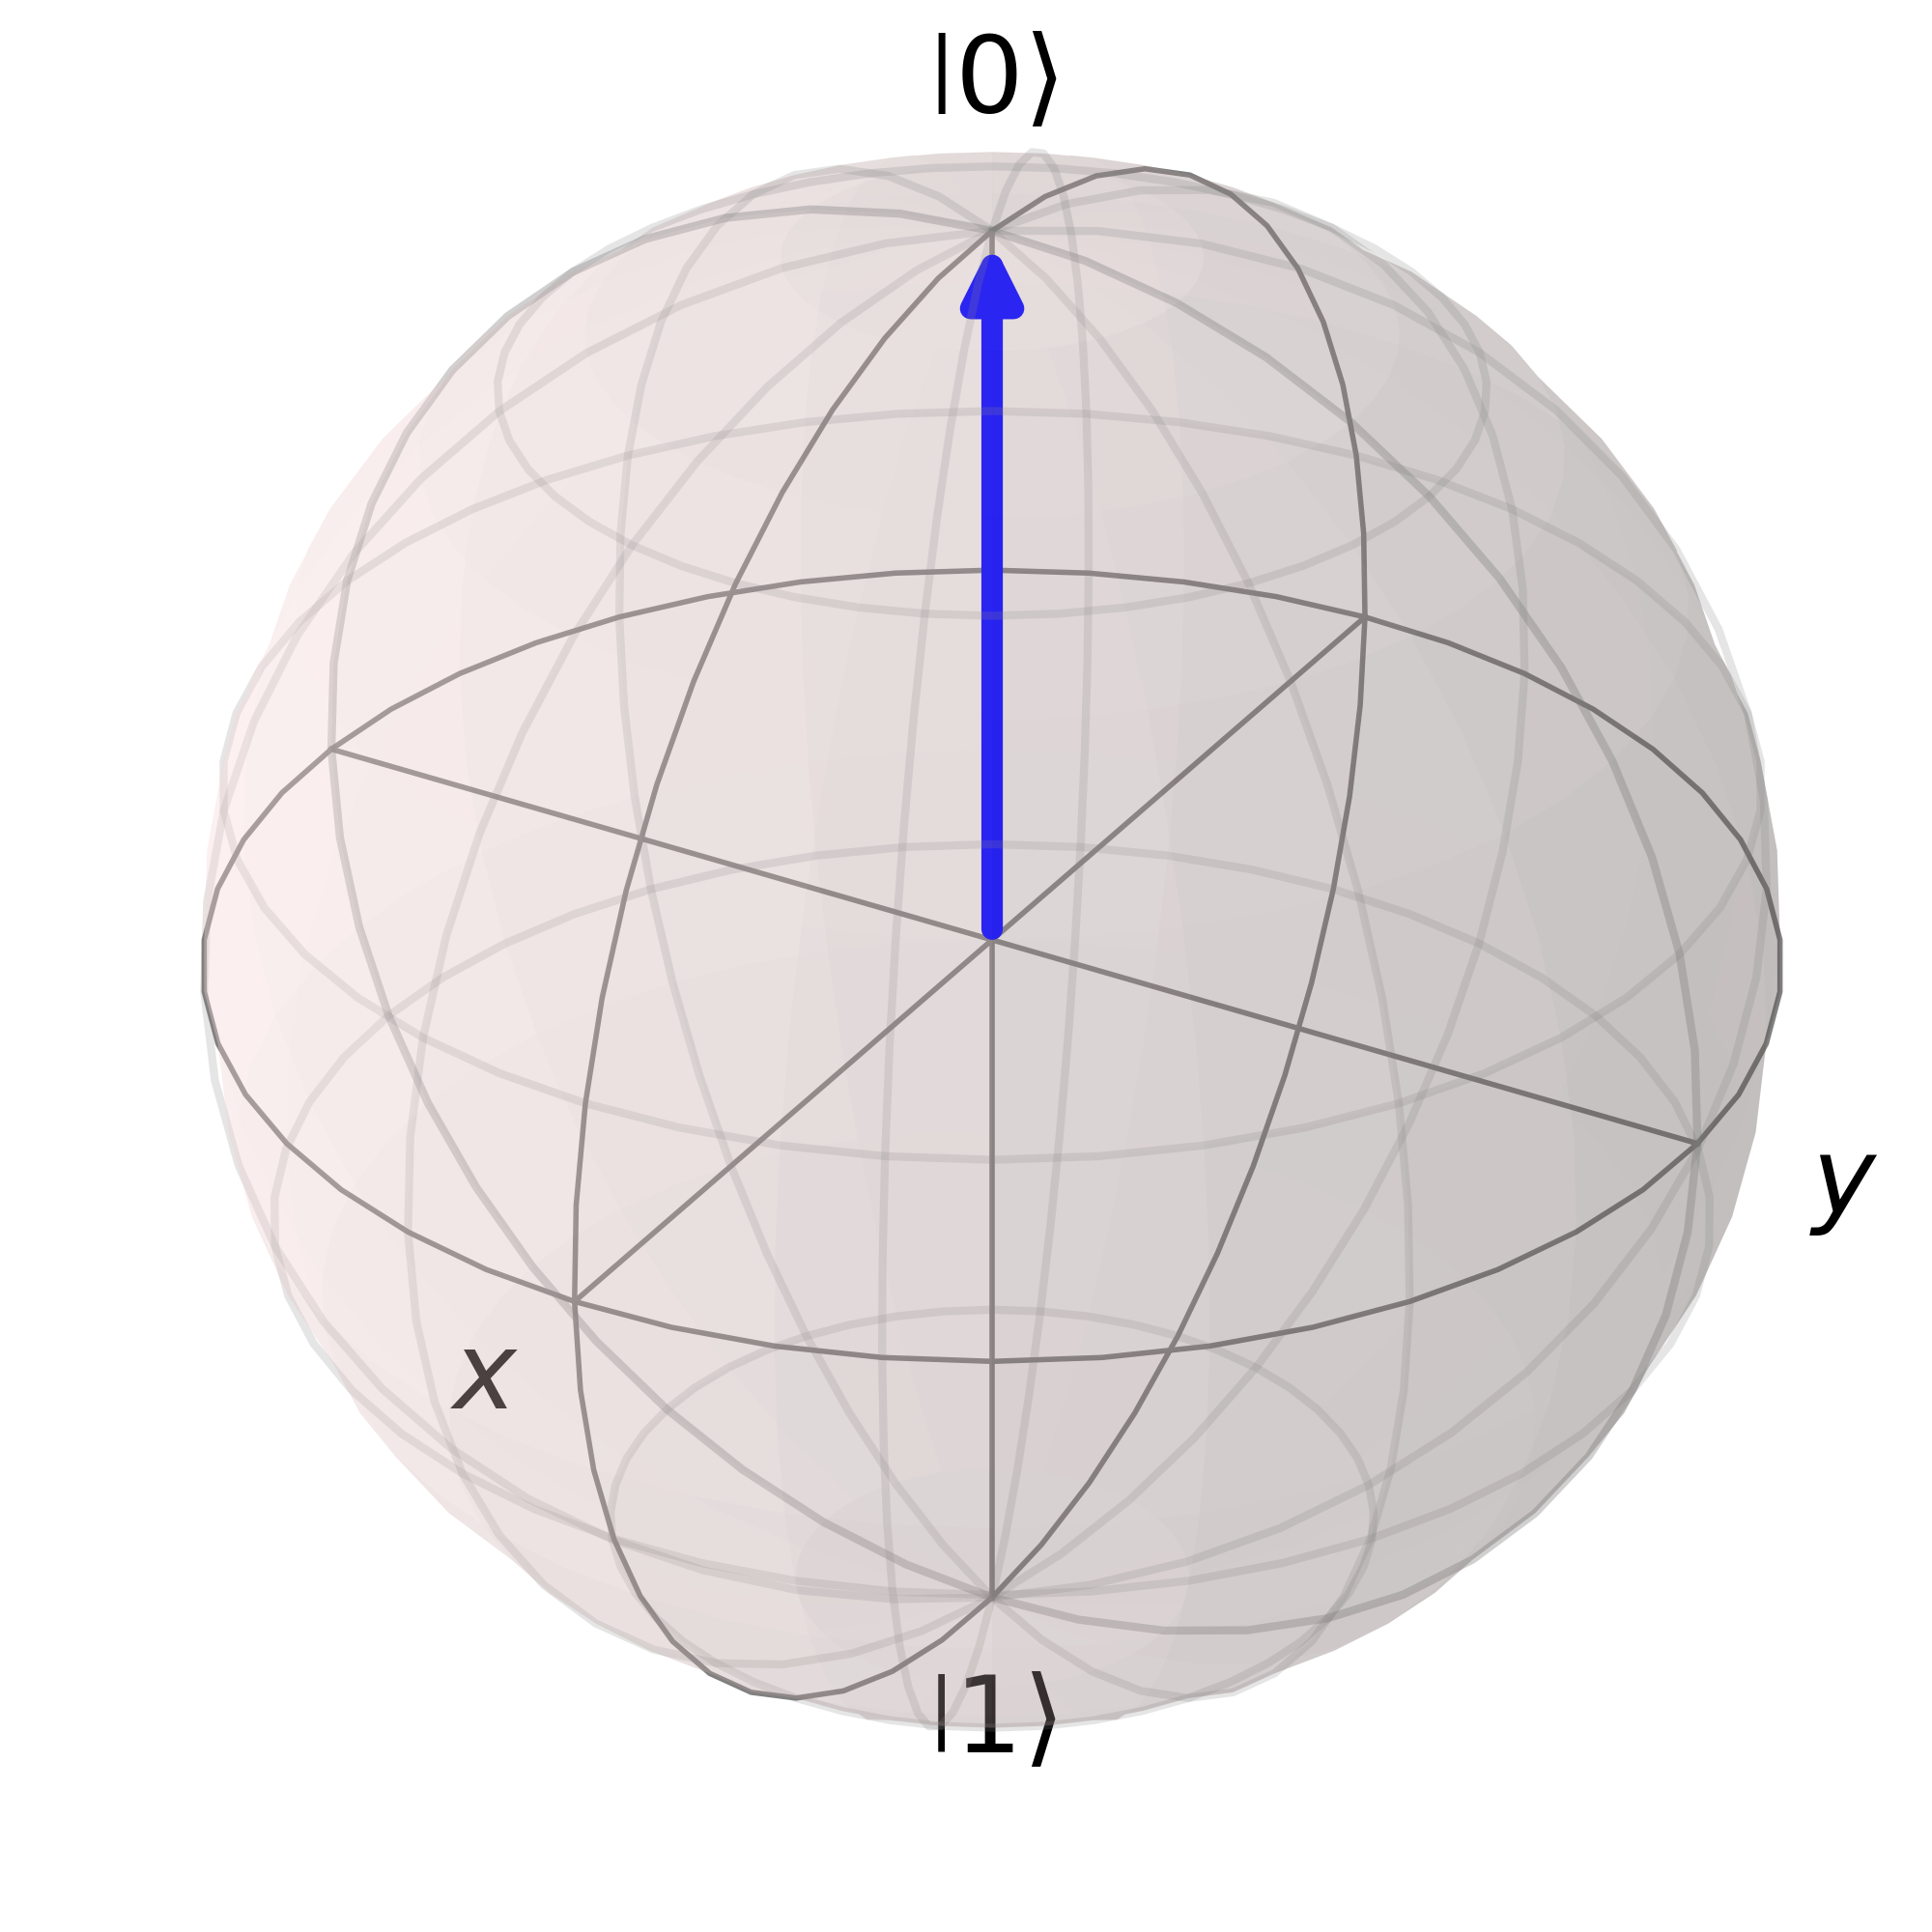
\includegraphics[width=0.5\textwidth]{qubit-zero-state.png}
       \caption{Príklad kostry grafu.}\label{fig:kostra}
    \end{center}
  \end{figure} 
\todo{cover what is initial state}
\textcolor{red}{TODO: global and relative phase may be also helpful}

\subsection{Quantum gates}
Quantum gates are operations that act on qubits. They are the quantum equivalent of classical logic gates. In contrast to logical gates in classical computing, quantum gates are represented by unitary matrices. \todo{add somewhere a definition of unitary matrix}.

One specialty of quantum gates is that they are reversible. This means that we can from the output of the gate, we can always determine the input. This is not the case for classical gates. For example, the logical AND gate is not reversible. From the output, we cannot determine the input.

Below are some of the most common quantum gates that are used in quantum computing.
\todo{if we use some of the gates that are not mentioned, we should add them here}
\todo{mention that some gates act on a single qubit, some on multiple qubits}
\todo{we can create arbitrary operation, just the matrix must adhere some properties}
\subsubsection{X gate}
The X gate is a single qubit gate. It is also known as a bit-flip gate because state $\ket{0}$ is flipped to $\ket{1}$ and vice versa. In simple words, it flips the state by 180 degrees around the x-axis of the block sphere.

% \begin{figure}[ht]
%     \centering
%     \begin{minipage}{0.4\linewidth}
%       \centering
%       $\begin{pmatrix}
%         0 & 1 \\
%         1 & 0
%         \end{pmatrix}$
%       \vfill
%     \end{minipage}
%     \hfill
%     \begin{minipage}{0.15\linewidth}
%       \centering
%       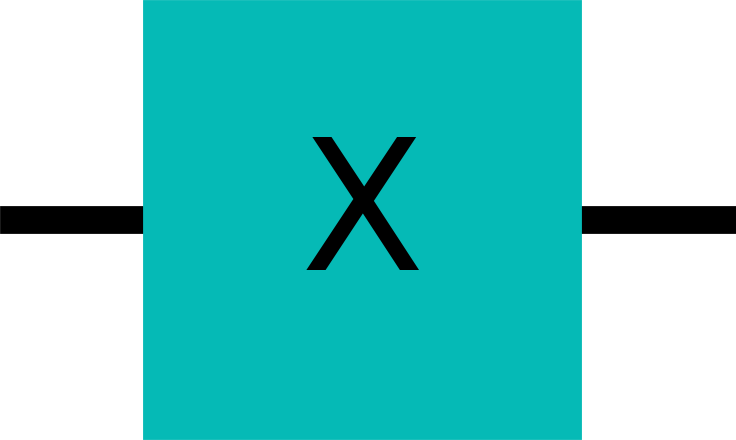
\includegraphics[width=\linewidth]{x-gate-icon.png}
%       \vfill
%     \end{minipage}
%     \caption{Matrix and visual representation of the X gate.}
% \end{figure}


\qubitRotation{qubit-zero-state.png}{qubit-x-gate.png}{X gate acting on initial state}

\subsubsection{Y gate}
\qubitRotation{qubit-zero-state.png}{qubit-y-gate.png}{Y gate acting on initial state}

\subsubsection{Z gate}
\qubitRotation{qubit-superposition.png}{qubit-z-gate.png}{Z gate acting on superposition state}
Note that this time we used a different initial state. If we used the previously the $\ket{0}$ state, we would not see any change.
\subsubsection{Hadamard gate}
\subsubsection{CNOT gate}
\subsection{Superposition}
\subsection{Measurements}
\subsection{Quantum entanglement}
\todo{consider the definition of unitary and hermitian matrices}
\textcolor{red}{TODO: reversibility, logical AND does not have an inverse function...}